\chapter{Simulation in RobotStudio}\label{chap:simulation}
A simulation in RobotStudio \cite{robotStudio} is used to check the algorithm without the need of a real robot cell. Since it is a dedicated ABB robot simulator, an ABB robot is used instead of the KUKA robot corresponding to the real setup. In any case, both are 6DOF robot arm that can be treated almost equally with some changes in the interface between MATLAB and the robot. 

A virtual cell similar to the real one is created containing the ABB robot arm, a table that defines the base workspace and Lego bricks. An image of the simulation station can be seen in \autoref{fig:sim_setup}.
\begin{figure}[H]
    %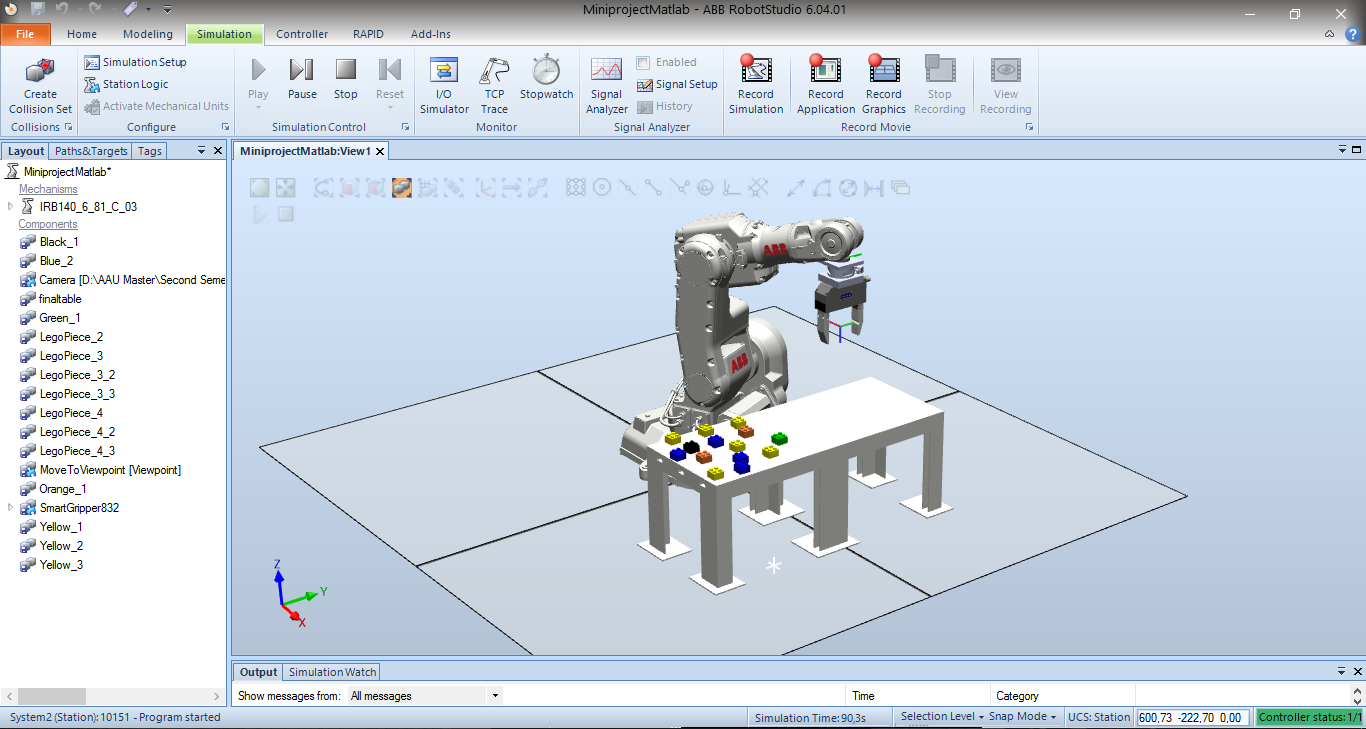
\includegraphics[width=0.25\textwidth]{figures/sim_setup.png}
    \caption{Simulation cell in RobotStudio used to reproduce the real cell.}
    \label{fig:simSetup}
\end{figure}

The robot used is a \fxnote{write model used} and it has a gripper attached to it to be able to pick the Lego bricks. The gripper is designed as a smart object in RobotStudio using a body with two fingers attached that can move. The fingers also contain a sensor that is used to know when a object has been grabbed by the gripper.

The table that defines the base workspace has a coordinate frame attached to one of its corners, see \autoref{fig:sim_setup}, with a position of (411.69,-285.27,340.12) with respect of the world frame of the robot and aligned with it. The position of the bricks is calculated with respect to the table frame and then the offset is added as in the case of the real robot.

The interface with the robot controller is done through MATLAB as well. This provides an easier integration of the vision algorithms and the robot movement. A MATLAB class, \lstinline[style=matlabinline]{RobotStudioConnector.m}, connects to the robot controller and defines the functions needed to operate the manipulator. The only difference is that in this case, the orientation is given in quaternions, so the angle needs to be transformed before sending the command. The used functions in the case of the simulation can be seen in \autoref{MatlabFunctionsSim}.

\begin{lstlisting}[ language = Matlab,
caption  = {Matlab functions used to operate the ABB robot in RobotStudio.},
label    = MatlabFunctionsSim ]
% Constructor of the class
robot = RobotStudioConnector(hostAddress_,hostPort_);
% Move to point with position (x,y,z) and orientation (q1,q2,q3,q4) in a linear motion
robot.moveLinear(x,y,z,q1,q2,q3,q4,speed)
% Open gripper
robot.gripperOn;
% Close gripper
robot.gripperOff;
\end{lstlisting}

The simulation station and a video with the results can be found in the attachment. 
As can be seen in the video, the identification of the brick's position and orientation work as expected and the robot is able to pick and place the bricks. 

The gripper is not the one used in the real robot and it has some problems when picking the bricks since it is not able to help the brick to position itself while grabbing it. For that reason the final figures are not fully aligned in the simulation. Nevertheless, in the case of the real robot, the gripper is made such that the block is always in the same position when it is grabbed so the final figures are mounted correctly.
